\documentclass[11pt, a4paper]{report}

\usepackage[utf8]{inputenc}
\usepackage[T1]{fontenc}
\usepackage[french]{babel}

% Appel des packages dans le dossier preambule
\def\packagepath{../../../../../preambule}   % path du package princial

\usepackage{\packagepath/page_layout} % <--- Nouveau
\usepackage{\packagepath/config_info}
\usepackage{\packagepath/cadres_cours}
\usepackage{\packagepath/zones_reponse}
\usepackage{\packagepath/config_ds}
\usepackage{\packagepath/config_maths}

% --- PILOTAGE ---
%\def\visibleornot{visible}    % visible or invisible
\ifdefined\visibleornot\else\def\visibleornot{visible}\fi


\def\documentpath{./Sources_Latex}
\graphicspath{{./Images/}}


\def\ptsexoA{0}



\begin{document}

\def\level{Premiere}  % Classe à droite
\def\course{NSI}
\def\chaptername{Les réseaux -- Adresses IP} % Titre au centre
\def\docname{ARSE05~--~TD 1}        % Identifiant à gauche

\pagestyle{DS_LP}

\NomPrenom{}

\begin{exercice_cours}[Quelques questions rapides]{}
    
On considère l'adresse IP suivante : \texttt{192.168.2.4} avec un masque de sous-réseau de \texttt{255.255.255.0}.
    \begin{enumerate}
        \item De quoi est composé une adresse IP? \hfill
        \item A quoi sert un masque de sous-réseau? 
        \item  Identifier la partie réseau et la partie hôte de cette adresse IP. \hfill
        \item Identifier l'adresse de réseau et l'adresse de diffusion (broadcast). \hfill
        \item La machine d'adresse IP \texttt{192.168.2.8} appartient-elle au même réseau que la machine d'adresse IP?
        \item La machine d'adresse IP \texttt{192.168.4.2} appartient-elle au même réseau que la machine d'adresse IP?
        \item Quel est le nombre maximum de machines pouvant être connectées sur ce réseau local? \hfill
    \end{enumerate}
\end{exercice_cours}

\begin{exercice_cours}[Notation CIDR]{}

    On considère l'adresse IP suivante : \texttt{192.168.25.120/20}.
    \begin{enumerate}
        \item Que signifie la notation CIDR? \hfill
        \item Identifier la partie réseau et la partie hôte de cette adresse IP. \hfill
        \item Identifier l'adresse de réseau et l'adresse de diffusion (broadcast). \hfill
        \item Quelle est la plage d'adresses IP disponibles pour les machines sur ce réseau local? \hfill
        \item Quel est le nombre maximum de machines pouvant être connectées sur ce réseau local? \hfill
    \end{enumerate}
\end{exercice_cours}

\begin{exercice_cours}[Interconnection de réseaux]{}

\begin{center}
    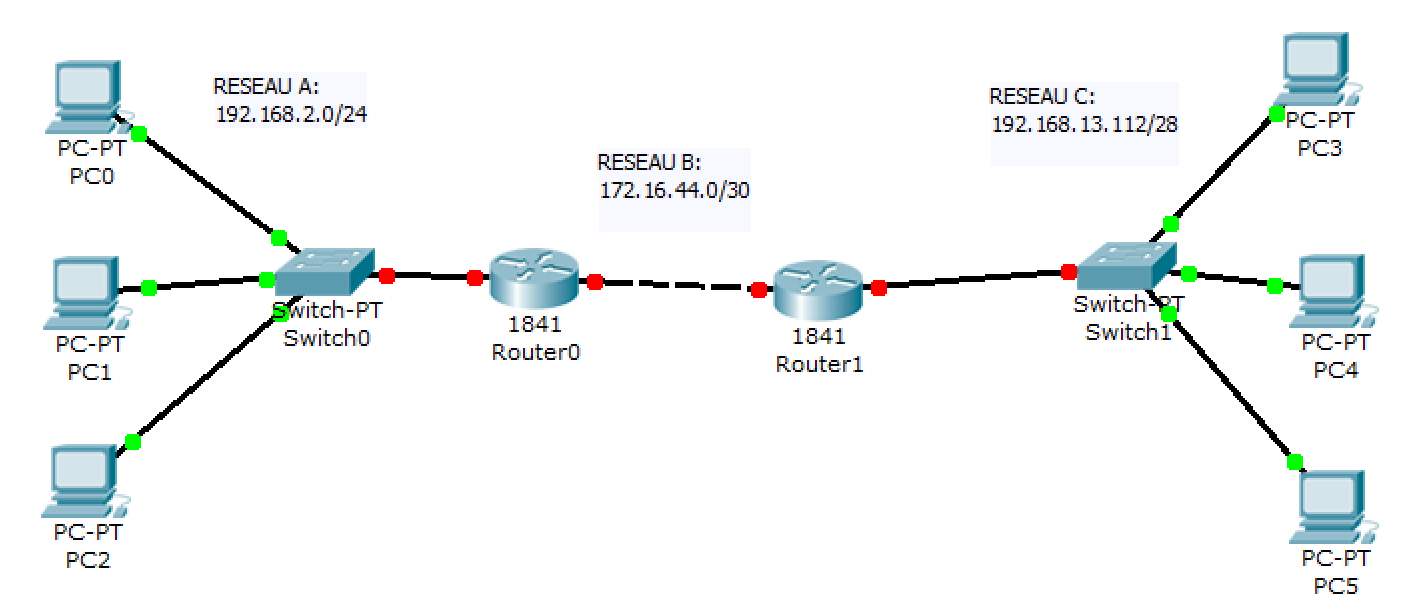
\includegraphics[width = 0.9\linewidth]{2026-06-09 15_41_53-Cisco Packet Tracer.png}
\end{center}

Les règles sont les suivantes:
\begin{enumerate}
    \item Les machines d'un même réseau local doivent pouvoir communiquer entre elles.
    \item Les machines d'un même réseau local doivent pouvoir communiquer avec les machines des autres réseaux locaux.
    \item les passerelles doivent pouvoir communiquer entre elles.
    \item les adresses IP des machines d'un même réseau local doivent être différentes.
    \item les adresses IP des passerelles sont toujours les dernières adresses disponibles d'un réseau local.
    \item les adresses IP des machines d'un même réseau local sont toujours les premières adresses disponibles d'un réseau local.
\end{enumerate}

\bigskip

     Proposer une configuration d'adresses IP, de masque et de passerelle pour les machines et les passerelles de ce réseau. \hfill
\end{exercice_cours}

\end{document}